\documentclass[11pt]{article}  
\usepackage[T1]{fontenc}
\usepackage[utf8]{inputenc}
\usepackage{helvet}
\usepackage{titlesec} 
\usepackage[frenchb]{babel}
\usepackage{amsmath,amssymb}
\usepackage{tabu}
\usepackage[svgnames]{xcolor}
\usepackage{graphicx}
\usepackage{geometry}
\usepackage{layout}
\usepackage{listings}
\usepackage{textcomp}
\usepackage{minted}
\usepackage{pdfpages}
\usepackage{fancyhdr}
\usepackage{lastpage}

\newenvironment{strechpage}[1][0cm]{%
	\newpage\vspace*{#1}\leavevmode\noindent\centering
	\def\tempdimen{#1}%
	\begin{minipage}{\dimexpr\linewidth-#1-#1\relax}}%
	{\end{minipage}\vspace*\tempdimen\newpage}
	
\pagestyle{fancy}
\renewcommand\headrulewidth{1pt}
\fancyhead[L]{TER: Calcul GRID avec de la messagerie instantanée}
\fancyhead[R]{URCA}
\renewcommand\footrulewidth{1pt}
\fancyfoot[L]{HERARD Joffrey}
\fancyfoot[C]{
\textbf{Page \thepage/\pageref{LastPage}}}
\fancyfoot[R]{2016-2017}



\titleformat{\chapter}[display]
  {\centering\normalfont\huge\bfseries}
  {\chaptertitlename\ \thechapter}
  {20pt}
  {\Huge}
  
\newcommand\T{\rule{0pt}{2.6ex}}       % Top strut
\newcommand\B{\rule[-1.2ex]{0pt}{0pt}} % Bottom strut

\begin{document}
 \makeatletter
\def\maketitle{%
  \null
  \thispagestyle{empty}%
  \vfill
  \begin{center}\leavevmode
    \normalfont
    {\Huge \@title\par}%
    \vskip 3cm
    {\Large \@author\par}%
    \vskip 1cm
    {\Large \@date\par}%
  \end{center}%
  \vfill
  \null
  \cleardoublepage
  }
\makeatother
\title{Solution générique de calcul GRID exploitant des messageries instantanées
(Java / Python, XML, XMPP / IRC)}
\author{ Réalisé par Joffrey Hérard \begin{center}Responsable : Olivier Flauzac\end{center}}
\date{2016-2017}
\maketitle
 
\tableofcontents 

\newpage
\section{Introduction} 
Sujet : Solution générique de calcul GRID exploitant des messageries instantanées
(Java / Python, XML, XMPP / IRC)
Durant ce TER, il a été demandé la mise en place d'un système de calcul reparti entre plusieurs machines avec l'évaluation de possibilités d'exécutions ou non par la machine cible, il fallait aussi évaluer quels échanges allaient être réalisés par les acteurs durant une exécution type et ceci avec le protocole XMPP ou IRC. Il sera détaillé dans ce rapport l'ensemble des échanges ainsi que l'ensemble des gestions d'erreurs déployées. 

\section{Les Acteurs} 
Pour commencer, nous avons deux genres d'acteurs pour chaque travail différent disponible :
\begin{itemize}
\item Un fournisseur de travail/Provider, est unique pour chaque travail à l'instant t.
\item Des travailleurs/Workers, de 1 à n, n défini par le problème.
Chaque Provider est possiblement exécuté sur n'importe quel système d'exploitation  tout comme chaque worker.
\item Un serveur XMPP qui sert de support à la messagerie instantanée avec Openfire.
\end{itemize}
\newpage

\section{Les Échanges} 
Voici la liste des différents messages qui transitent à travers une exécution type.

 
\begin{enumerate} \item Nous avons en premier le message de type "ENVOI JOB", il contient :
\begin{itemize}
\item L'identifiant du problème,
\item Le code des contraintes,
\item Le code à exécuter,
\item La ligne de  commande pour l\textquoteright exécuter.
\item Le nom du fichier à exécuter.
\end{itemize}

\item Ensuite lorsque le worker est prêt, il le signale par un message qui contient juste dans une chaîne de caractère "Je suis prêt".
\item Il y a enfin le message qui renvoi le résultat "REPONSE JOB" celui-ci contient : 
\begin{itemize}
\item L'identifiant pour savoir si le code a pu être exécuté.
\item L'identifiant du problème.
\item La valeur du retour de l\textquoteright exécution.
\item Le Code de contraintes, si on a pas pu l'exécuter.
\item Le Code exécutable, si on a pas pu l'exécuter.
\item La Ligne de commande associée, si on a pas pu l'exécuter.
\item Le nom du fichier à exécuter.
\end{itemize}
\end{enumerate}
Voici la liste des fichiers schéma XML associés ainsi que leurs locations au sein du projet :
\begin{itemize}	
\item "ENVOI\_JOB" = ../Schema\_XML/ENVOI\_RECEPTION.xsd.
\item "REPONSE\_JOB"= ../Schema\_XML/JOB\_REP.xsd.

\end{itemize}



\newpage

 
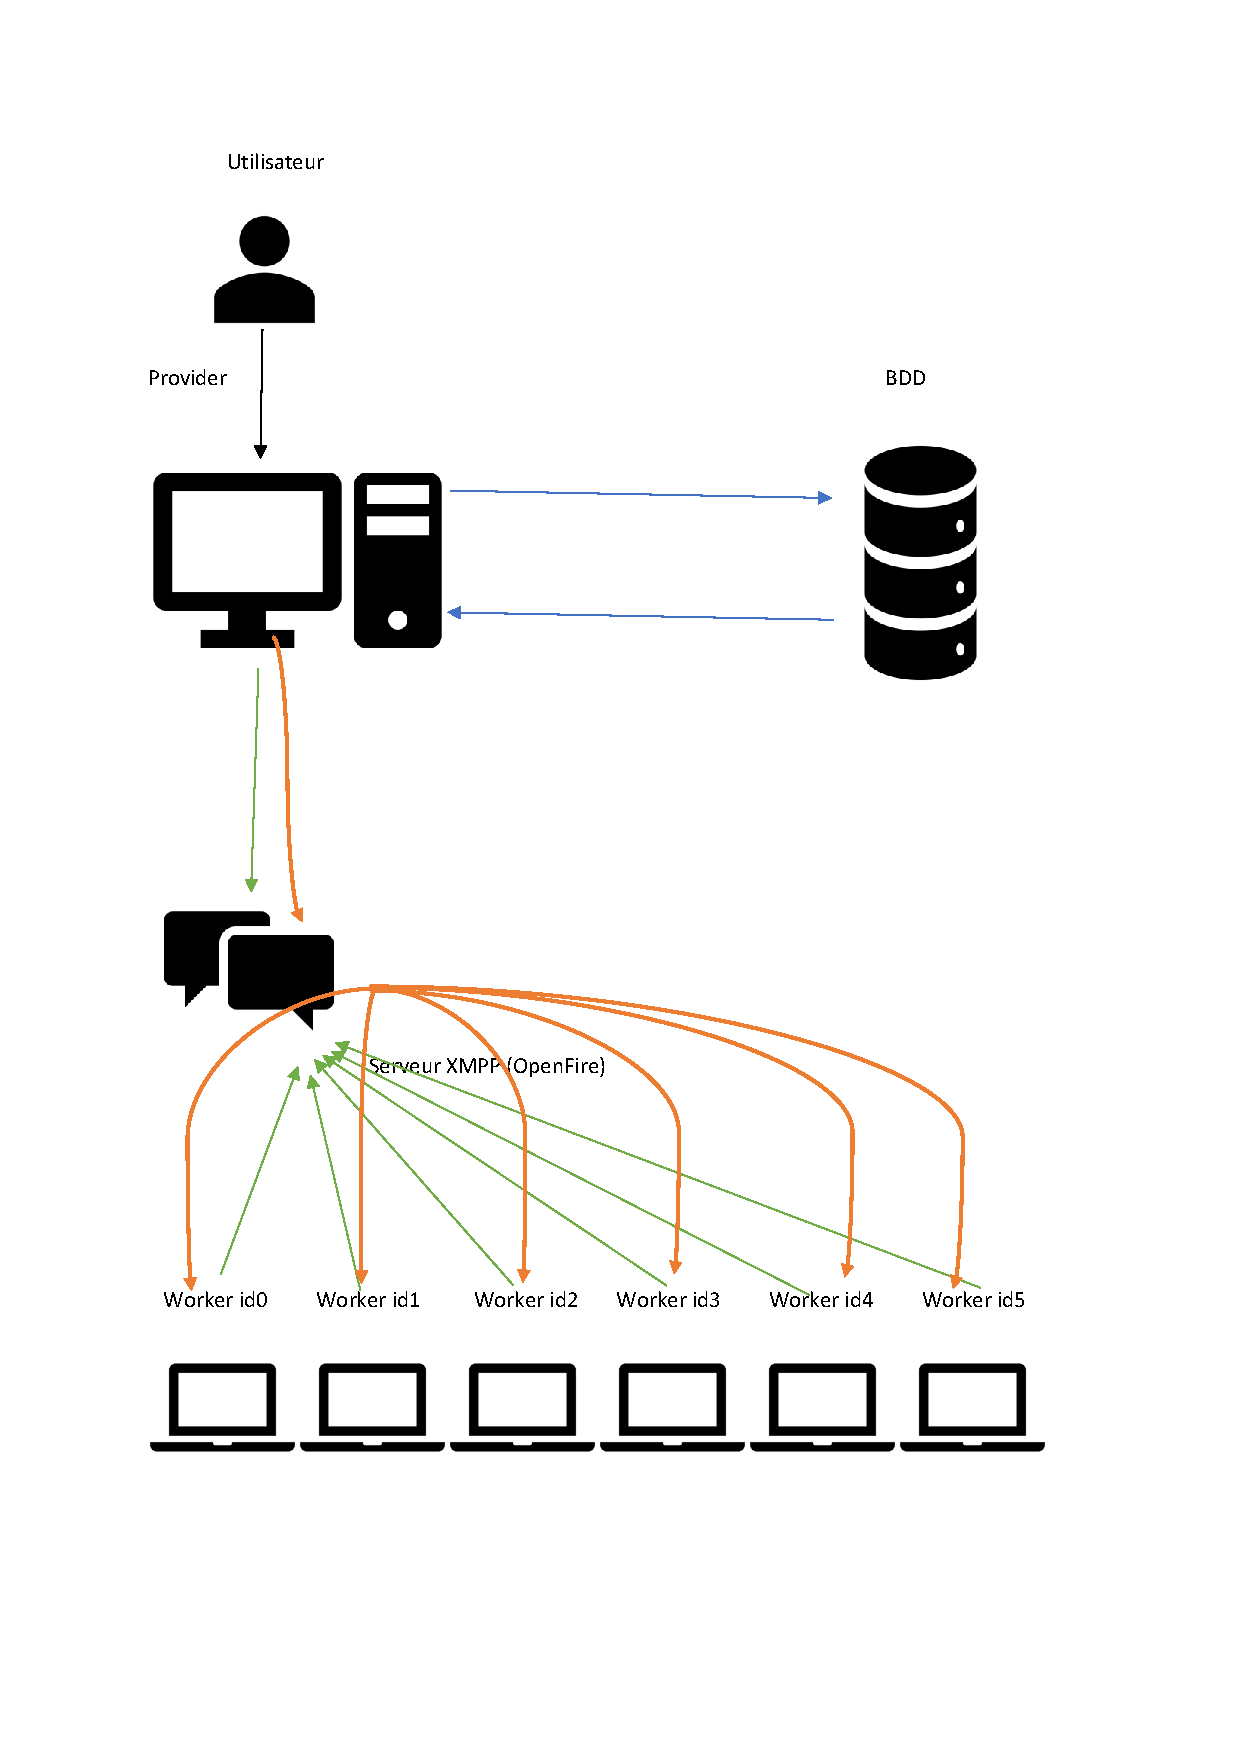
\includepdf[scale=0.7,pages=1,pagecommand=\section{Modélisation}\subsection{Schéma général}\subsubsection{Schéma global d'envoi d'un job}]{toto.pdf}
\includepdf[scale=1,pages=4]{toto.pdf}

\includepdf[scale=0.7,pages=2,pagecommand=\subsubsection{Schéma global d'envoi de réception d'un job}]{toto.pdf}
\includepdf[scale=1,pages=3]{toto.pdf}
\newpage
\subsection{Représentation des JOBS}
Nous allons dans cette partie du rapport montrer la représentation nécessaire et désirée pour représenter un travail. Donc qu'est-ce qu'un problème ?

\begin{itemize}
\item L'identifiant d'un problème, un entier de 0 à n.
\item Le code de contraintes, ce code est forcément un code Perl avec un code de retour bien particulier 0 pour non exécutable et 3 pour exécutable et donc que l'on peut exécuter. 
\item Le type du fichier par exemple ".c , .cpp, .cc, .java , .pl etc.."
\item Le code d'exécution : On peut l'exécuter si le code contraintes l'a validé et cela  peu importe son langage.
\item La ligne de commande pour exécuter le code, par exemple "perl monfichier.pl"
\end{itemize}

\inputminted{XML}{../Schema_XML/BDD_JOB.xsd}
\newpage 

\subsection{Représentation des fichiers de lignes de commandes} 
Chaque ligne de commande doit être représentée comme elle se doit de respecter ces 2 règles simples : 
\begin{enumerate}
\item Après la commande de type perl, python. ./, il doit être suivi d'un @,  
\item La commande puis une ','
\end{enumerate}
Si ces règles ne sont pas respectées, le "parsing", se faisant sur ce fichier par une expression régulière, ne s\textquoteright appliquera pas correctement  
\inputminted{perl}{../Echantillon_Script_Cmd/Toto.dc}
Exemple de Langford\_mono12.dc :
\inputminted{perl}{../Echantillon_Script_Cmd/Langford_mono12.dc}
Exemple de nQueen14.dc :
\inputminted{perl}{../Echantillon_Script_Cmd/nQuenn14.dc}

La raison principale de la présence de l'arobase c'est qu'il va falloir reconstruire la ligne de commande pour ajouter le chemin correspondant.
La raison de la présence de la virgule c'est la ligne de commande personnalisée d'un worker séparée d'une autre.
\newpage
\subsection{Les différentes fonctions principales}

\subsubsection{Contraintes} 
L'exécution d'un script de contrainte se fait avec les objets Runtime et Process, on obtient le résultat du script avec la fonction waitFor() 
\inputminted{perl}{../Echantillon_Script_Perl/OSname.pl}
\newpage
\subsubsection{Séparation} 
La fonction split peut se résumer en plusieurs étapes : Dans un premier temps, on récupère tous les nicknames et JIDs de chaque utilisateur de la chatroom, pour chacun d'entre eux on leur envoi un fichier XML personnalisé avec chacun une tâche bien distincte en respectant le schéma associé. Pour avoir une trace on sauvegarde chaque fichier xml envoyé dans le dossier JOB\_SEND
\inputminted[tabsize=2,frame=lines,linenos]{java}{Fichier_import/split.java}
\subsubsection{Exécution} 
L\textquoteright exécution d'un script d'exécution se fait avec les objets Runtime et Process, on attend le résultat du script avec la fonction waitFor() et bien entendu on a un résultat chiffré dans un fichier. 
\inputminted[tabsize=2,frame=lines,linenos]{Perl}{Fichier_import/calcul.pl}
\newpage
\subsubsection{Construction du résultat} 
La fonction build est simplement une addition de chaque résultat reçu petit à petit 
\inputminted[tabsize=2,frame=lines,linenos]{java}{Fichier_import/build.java}
\newpage
\subsection{Description d'une exécution quelconque} 
\subsubsection{Exécution cote Provider}
Voici un déroulement classique coté Provider :
\begin{enumerate}
\item Un Provider choisi un problème à lancer.
\item Une fois le problème lancé une Chatroom comportant le nom du problème+Providingroom est créée sur le domaine.
\item Le Provider attend un nombre suffisant de Workers en fonction du problème (champ rang du XML).
\item Une fois ce nombre atteint, on récupère chaque identifiant et on envoi à chaque worker son job ainsi que la ligne de commande.
\item On attend d'avoir reçu un message de type "JOB\_Reponse" autant de fois que de Workers capablent de l'exécuter. 
\item On affiche enfin le résultat. 
\end{enumerate}

\subsubsection{Exécution cote Worker}
Voici un déroulement classique coté Worker
\begin{enumerate}
\item On s'identifie.
\item On choisi une salle de travail .
\item Une fois connecté on applique la même routine 
: A savoir, on exécute chaque script de contrainte, si ils sont validés, on exécute le fichier exécutable avec la ligne de commande associée.
\end{enumerate}
\subsubsection{Exécution d'un ajout}
\begin{enumerate}
\item On demande le nom du problème.
\item On demande en entrée le chemin absolu pour un fichier de contrainte.
\item On demande en entrée le chemin absolu pour un fichier exécutable.
\item On demande en entrée le chemin absolu pour un fichier correspondant aux lignes de commande.
\item On demande en entrée un rang qui est égal au nombre de workers nécessaires. 
\item Tout ceci est ajouté à un fichier XML nommé nom\_du\_probleme.xml
\end{enumerate}

\newpage\subsubsection{Exécution d'une suppression}
\begin{enumerate}
\item On demande le nom du problème. 
\item On supprime le fichier XMl associé. 
\end{enumerate}
\newpage
\section{Formatage des fichiers sources décrivant un JOB}
\subsection{Script de contraintes}
\subsubsection{Principe}
Tous scripts de contrainte doivent répondre à leurs propres contraintes :
\begin{enumerate}
\item Être écrit en Perl.
\item Avoir un retour de commande avec "exit(3);" pour un retour validant la poursuite du processus. 

\end{enumerate}
\subsubsection{Exemple}
\subparagraph{Exemple pour un programme interprété}
Pour un langage interprété comme le python en voici un exemple :
\inputminted{perl}{../Echantillon_Script_Perl/nqueen.pl}
\subparagraph{Exemple pour un programme compilé }
Quand il s'avère que vous devez valider la compilation puis sa future exécution d'un code exécutable tel qu'un code de langage compilé comme le C en voici un exemple pour connaître la démarche  à suivre.  
\inputminted{perl}{../Echantillon_Script_Perl/langford.pl}
\subsection{Script de Commandes}
\subsubsection{Principe}
Cette partie fait aussi une référence, voire une redite avec le section 5-3. Tous scripts de commande doivent répondre à leurs propres contraintes :
\begin{enumerate}
\item Après la commande faisant appel à un interpréteur mettre le caractère "@".
\item Dans le cas d'un split à plus de un Worker, utilisez les virgules pour séparer chaque commande appropriée pour chaque Worker.
\item Les caractères évidemment interdits sont :<< @, ',', [, ] >>. En raison d'exploitations d'expressions régulières.
\end{enumerate}
\subsubsection{Exemples}
Voici quelques exemples :
\inputminted{perl}{../Echantillon_Script_Cmd/nQuenn14.dc}
\inputminted{perl}{../Echantillon_Script_Cmd/Toto.dc}

\subsection{Script d'exécution}
\subsubsection{Principe}
Tous scripts des exécutions doivent répondre à leurs propres contraintes :
\begin{enumerate}
\item Avoir connaissance que toutes les données renvoyées par les Worker seront passées dans le fichier résultat.
\item Écrire le résultat dans un fichier "resultat.txt".
\end{enumerate}


\subsection{Script de build}
\subsubsection{Principe}
Tous scripts de construction doivent répondre à leurs propres contraintes :
\begin{enumerate}
\item Être écrit en Perl.
\item Avoir connaissance que toutes les données renvoyées par les Workers seront passées en argument.
\item Écrire le résultat dans un fichier "resultatF.txt".
\end{enumerate}
\subsubsection{Exemple}
\inputminted{perl}{../Echantillon_Script_build/build.pl}
\newpage
\section{Contrainte du serveur OpenFire }
Il est nécessaire, afin que le programme fonctionne, que le serveur soit accessible par tout le monde de là où il se trouve, il est possible de demander une machine virtuelle avec un serveur OpenFire (ou autre d’ailleurs) tant qu'il est possible pour un provider d'y être inscrit par un administrateur au grade de modérateur, respectivement pareil pour un worker. 
Il est important de savoir que là il y a plusieurs limite de OpenFire.
\newpage
\section{Les Erreurs} 
\subsection{Les Problèmes d'exécution}
Les problèmes qui peuvent opérer à travers le système sont : 
\begin{enumerate}
\item Un mauvais nom de domaine. 
\item Un problème de Chatroom déjà existante.
\item Un problème d'exécution : aucun worker ne peut exécuter le code, comment le détecter ?

\end{enumerate}  

\newpage
\subsection{Les Problèmes réseau}
Nous avons plusieurs problèmes liés au réseau quelque soit le protocole utilisé :
\begin{enumerate}
\item Latence/Impossible à établir une connexion à la Chatroom.
\item Latence/Impossible à envoyer un  message d'un Provider vers un Worker.
\item Latence/Impossible à envoyer un  message d'un Worker vers un Provider.
\item Un Worker est déconnecté en plein milieu de sa tâche.
\item Un Provider est déconnecté durant l'attente d'une réponse sur un JOB.
\end{enumerate}


\newpage
\subsection{Gestions des erreurs}

\subsubsection{Gestions des erreurs sur l\textquoteright exécution}
\begin{enumerate}
\item Mauvais nom de domaine $ \rightarrow $ Redemander le nom de domaine jusqu'à validation.
\item Problème de ChatRoom déjà existante $\rightarrow$ Message d'erreur un problème exactement identique est en cours d'exécution.
\item Problème d'exécution : aucun worker ne peut exécuter le code, comment le détecter ? $\rightarrow$ Mise en place d'un tableau de variable booléenne au départ initialisé à faux, si un worker renvoi avec une impossibilité d\textquoteright exécution du code dicté par le code contrainte, alors on met à vrai et on redistribue. Si aucun n'est capable on arrête l\textquoteright exécution.
\end{enumerate}  
\subsubsection{Gestions des erreurs sur le réseau}
\begin{enumerate}
\item Latence/Impossible à établir une connexion à la ChatRoom$ \rightarrow $ Message qui explicite le fait d'aller voir un Administrateur Réseau.
\item Latence/Impossible à envoyer un message d'un Provider vers un Worker$ \rightarrow $ Message qui explicite le fait d'aller voir un Administrateur Réseau.
\item Latence/Impossible à envoyer un  message d'un Worker vers un Provider$ \rightarrow $ Message qui explicite le fait d'aller voir un Administrateur Réseau. 
\item Un Worker est déconnecté en plein milieu de sa tâche$ \rightarrow $ Détecteur de présence permis par le protocole XMPP sur une ChatRoom MultiUser.
\item Un Provider est déconnecté durant l'attente d'une réponse sur un JOB$ \rightarrow $ Évaluation de présence d'un Provider, si aucun alors arrêter le Job en cours, ou mise en place d'un TimeOut.
\end{enumerate}

\newpage
\section{Conclusion}
Cette conclusion sera séparée en plusieurs parties : la première concernant l'aspect des problèmes qui resteraient à gérer. La deuxième partie sera concentrée sur la partie XMPP, la troisième sur les jobs à entrevoir, et la quatrième sur une virtualisation des services. Pour finir cette conclusion, un retour sur le TER.
\subparagraph{Les problèmes qu'il reste à gérer}
\begin{enumerate}
	\item Comment résoudre une perte réseau de longue durée sur un worker, quelle serait la pertinence d'un envoi de résultat après un certain temps ? 
	\item Avoir des informations de disponibilité de la bande passante du serveur hôte de messagerie instantanée si l'on souhaite avoir des communications en temps réel.
	\item Si le Provider de JOB tombe en panne pendant les calculs que faire, que ce soit un problème réseau ou électrique ?
\end{enumerate}
\subparagraph{OpenFire}
\begin{enumerate}
\item Il reste à évaluer les besoins et la montée en charge associés au serveur XMPP. Il aurait été plus intéressant lors de mes tests, d'utiliser un serveur XMPP externe pour lui faire éprouver des stress tests. Ainsi donc en voir des éventuelles limites qui apporteraient de nouveaux problèmes à gérer.
\item Il y a des machines virtuelles avec des serveurs XMPP déjà configuré c'est une voie qu'il reste à exploiter.
\end{enumerate}

\subparagraph{JOB à entrevoir} 
Comme nous en avons déjà parlé durant quelques entrevues, il reste un point sur lequel je n'ai pu me pencher : une utilisation par exemple de l'outil POV-ray ou des tabulations de Golomb. Respectivement, POV-ray s'utilisant en lignes de commandes, seul le support de travail reste à définir, les tabulations de Golomb sont particulières, elles restent du domaine du calculatoire sur les espacements de blocs. 
\subparagraph{Virtualisation des services}
Une possibilité qui techniquement était envisageable sur ce sujet de TER, il est possible de lancer des conteneurs par exemple avec Docker. Évidemment l’intérêt serait d'avoir des machines personnalisées avec les outils qui serait intéressant. Tout cela j'ai pu les envisager avec l'aide de Guillaume Bourgeois, qui m'a conseillé sur la manière de les gérer, je n'ai évidemment pas développé en profondeur cela dans le désir de ne pas empiéter sur son sujet.
\subparagraph{En résumé} 
Le sujet avait beaucoup d'aspects à couvrir, bien entendu tout l'aspect réseau, pour la transmission des messages, l'aspect programmation pour s'adapter aux API XMPP disponibles, et bien entendu l'aspect d’études sur les échanges, et la montée en charges des besoins pour le serveur XMPP.

\newpage

\section{Annexes}
\subsection{Organisation du dossier du projet}
\begin{itemize}
\item / \begin{itemize}
		\item /bin  \begin{itemize} \item Tout les fichiers .class \item Images \item Schema    \end{itemize}
		\item /DB\_JOBS \begin{itemize} \item Calculatoire.xml \item LangfordMono12.xml \item NQueenMono8build.xml \ \item Tout les probleme.xml \end{itemize}
		\item /Echantillon\_Script\_Cmd \begin{itemize} \item Toto.dc \item nQueen14.dc \item Langford\_mono12.dc\item Tout les probleme.dc\end{itemize}
		\item /Echantillon\_Script\_Exec \begin{itemize}\item calcul.pl \item Langford(Dossier comportant les fichiers exemple sur langford) \item nQueen(Dossier comportant les fichiers exemple sur nqueen)  \end{itemize}
		\item /Echantillon\_Script\_Perl \begin{itemize}\item  OSname.pl \item nqueen.pl \item langford.pl\end{itemize}
		\item /JDOM  
		\item /JOB\_REC \begin{itemize}\item /DATA\_EXTRACT \begin{itemize} \item fichier\_extraits\end{itemize}\item xml\_receive.xml  \end{itemize}
		\item /JOB\_SEND \begin{itemize}\item XML\_send\_0.xml \end{itemize}
		\item /openfire
		\item /Rapport \begin{itemize}\item TER\_Joffrey\_Herard.pdf  \end{itemize} 
		\item /Schema\_XML \begin{itemize}\item BDD\_JOB.xsd \item ENVOI\_RECEPTION.xsd \item JOB\_REP.xsd \end{itemize}
		\item /smack\_3\_1\_0
		\item /src \begin{itemize}\item Tout les fichiers .java \end{itemize}
		\item README.md 
\end{itemize}

\end{itemize}
\newpage
\subsubsection{Outils et langages} 
\begin{enumerate}
\item Le projet a été programmé en Java version : "1.8.0\_111" sous Eclipse.
\item L'API smack a été utilisé pour mettre en place les échanges sous XMPP.
\item Openfire a été utilisé pour installer un serveur XMPP en local afin d'exécuter tous les test.
\end{enumerate}
\newpage

\newpage
\subsection{Code}
\subsubsection{XML} 

BDD\_JOB.xsd
\inputminted[tabsize=2,frame=lines,linenos]{XML}{../Schema_XML/BDD_JOB.xsd}

ENVOI\_RECEPTION.xsd
\inputminted[tabsize=2,frame=lines,linenos]{XML}{../Schema_XML/ENVOI_RECEPTION.xsd}
\newpage
JOB\_REP.xsd
\inputminted[tabsize=2,frame=lines,linenos]{XML}{../Schema_XML/JOB_REP.xsd}
\newpage
\subsubsection{Fichier de lignes de commande .dc}
Les exemple de fichier de commande écrit en texte clair 
Toto.dc
\inputminted[tabsize=2,frame=lines,linenos]{Perl}{../Echantillon_Script_Cmd/Toto.dc}
\subsubsection{Perl}
Les exemple de fichier de contrainte écrit en Perl 
langford.pl
\inputminted[tabsize=2,frame=lines,linenos]{Perl}{../Echantillon_Script_Perl/langford.pl}

nqueen.pl
\inputminted[tabsize=2,frame=lines,linenos]{Perl}{../Echantillon_Script_Perl/nqueen.pl}
OSname.pl
\inputminted[tabsize=2,frame=lines,linenos]{Perl}{../Echantillon_Script_Perl/OSname.pl}

\end{document}